\chapter{Results}\label{ch:Results}

CNO = 45

PLLBW =32
FLLBW = 10
76.135, std = 2.3549

PLLBW = 18
FLLBW = 1
128.26,std =  2.59 

PLLBW = 32
FLLBW = 0
131.6 std = 1.64

\begin{figure}[!htb] 
    \centering
    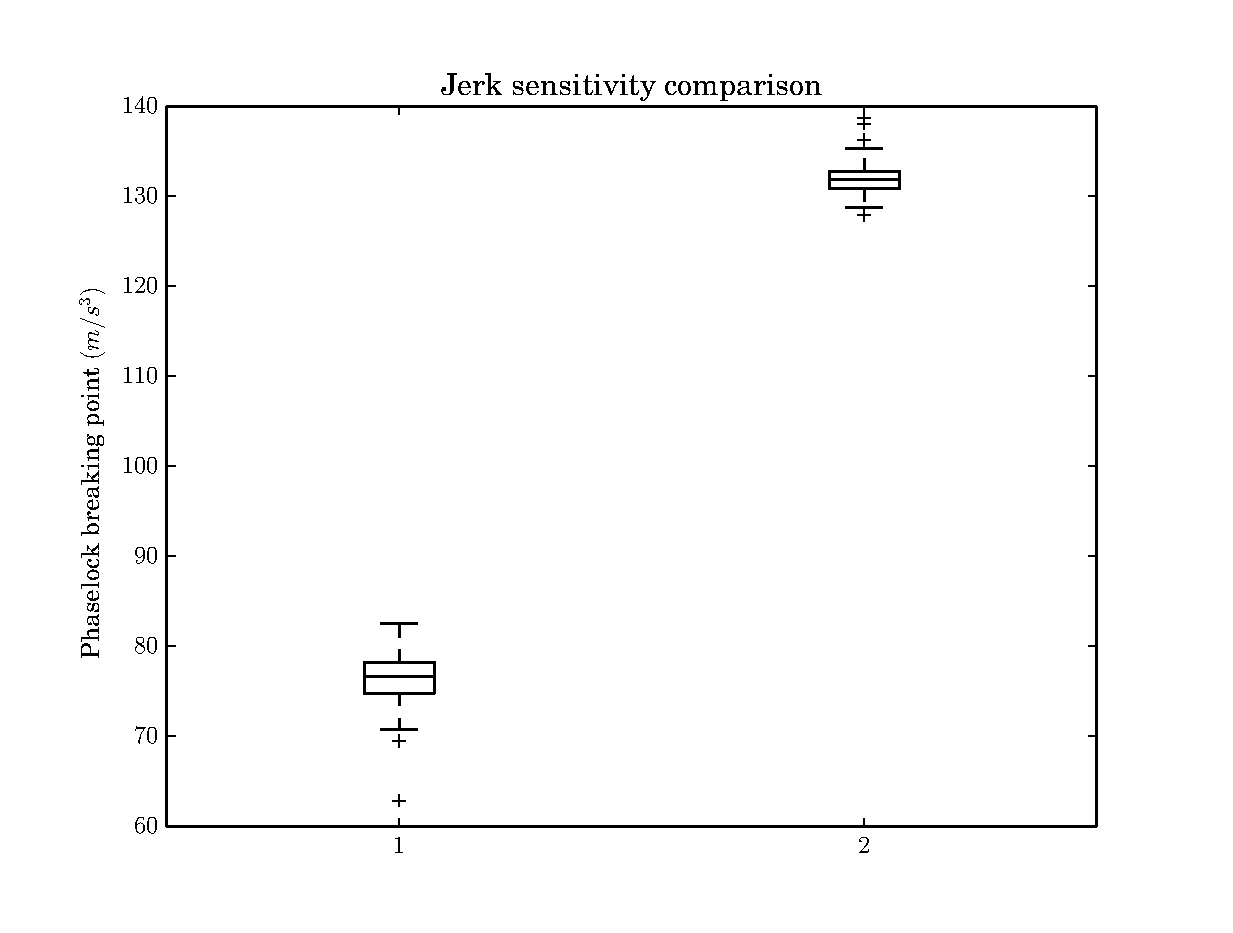
\includegraphics[width=1\textwidth]{mywork/BoxplotJerk.eps} 
    \caption{ 76.135, std = 2.3549 vs 131.6 std = 1.64}
    \label{fig:BoxplotJerk}
\end{figure}


\begin{figure}[!htb] 
    \centering
    \includegraphics[width=1\textwidth]{mywork/BoxplotPhaseJitter.eps} 
    \caption{5.77987052071 0.280738421289 vs 4.3143405835 0.0443823631819}
    \label{fig:BoxplotPhaseJitter}
\end{figure}

